\chapter{Abstract Factory模式}
\section{抽象工厂模式的概念}
抽象工厂(AbstractFactory)模式的定义:是一种为访问类提供一个创建一组相关或相互依赖对象的接口,且访问类无须指定所要产品的具体类就能得到同族的不同等级的产品的模式结构。
\begin{enumerate}
	\item 抽象工厂模式是工厂方法模式的升级版本,工厂方法模式只生产一个等级的产品,而抽象工厂模式可生产多个等级的产品。
	\item 抽象工厂的工作是将“抽象事件”组装为“抽象产品”。
	\item 抽象工厂不关心零件的具体实现,而是只关心接口(API),可以仅使用接口(API)将零件组装为产品。
\end{enumerate}
\subsection{应用条件}
\begin{itemize}
	\item 系统中有多个产品族,每个具体工厂创建同一族但属于不同等级结构的产品。
	\item 系统一次只可能消费其中某一族产品,即同族的产品一起使用。
\end{itemize}
注:抽象工厂模式的扩展有一定的“开闭原则”倾斜性:
\begin{itemize}
	\item 当增加一个新的产品族时只需增加一个新的具体工厂,不需要修改原代码,满足开闭原则
	\item 当产品族中需要增加一个新种类的产品时,则所有的工厂类都需要进行修改,不满足开闭原则。
\end{itemize}
\subsection{优点}
\begin{itemize}
	\item 可以在类的内部对产品族中相关联的多等级产品共同管理,而不必专门引入多个新的类来进行管理。
	\item 当增加一个新的产品族时不需要修改原代码,满足开闭原则。
\end{itemize}
\subsection{缺点}
当产品族中需要增加一个新的产品时,所有的工厂类都需要进行修改。
\section{抽象工厂的角色}
\begin{enumerate}
	\item 抽象工厂(Abstract Factory):提供了创建产品的接口,它包含多个创建产品的方法 newProduct(),可以创建多个不同等级的产品。
	\item 具体工厂(Concrete Factory):主要是实现抽象工厂中的多个抽象方法,完成具体产品的创建。
	\item 抽象产品(Product):定义了产品的规范,描述了产品的主要特性和功能,抽象工厂模式有多个抽象产品。
	\item 具体产品(ConcreteProduct):实现了抽象产品角色所定义的接口,由具体工厂来创建,它 同具体工厂之间是多对一的关系。
	\item 委托者(Client):Client仅会调用抽象工厂角色和抽象产品的接口,
	对于具体的零件、产品和工厂一无所知。
\end{enumerate}
\section{抽象工厂的结构}
\begin{figure}
	\centering
	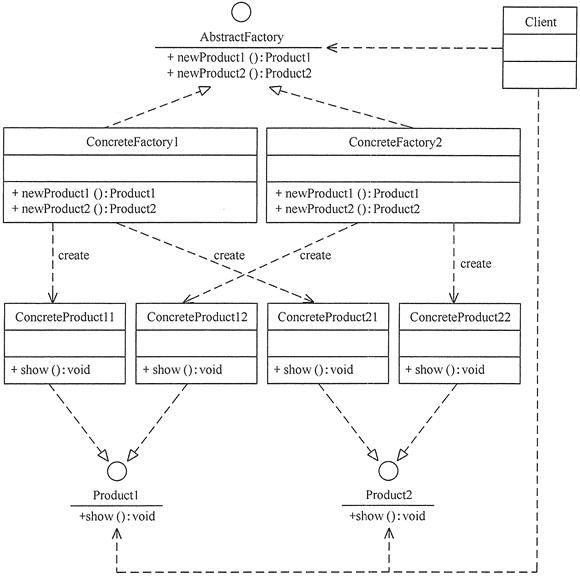
\includegraphics[width=0.8\textwidth]{image/8-2}
	\caption{抽象工厂模式的结构图}
\end{figure}
\section{抽象工厂实现——例一}
\begin{lstlisting}
//抽象工厂
interface AbstractFactory {
public Product1 newProduct1();
public Product2 newProduct2();
}
\end{lstlisting}
\begin{lstlisting}
//具体工厂
class ConcreteFactory1 implements AbstractFactory {
	public Product1 newProduct1() {
		System.out.println("具体工厂 1 生成-->具体产品 11...");
		return new ConcreteProduct11();
	}
	public Product2 newProduct2() {
		System.out.println("具体工厂 1 生成-->具体产品 21...");
		return new ConcreteProduct21();
	}
}
\end{lstlisting}
\section{抽象工厂实现——例二}
\begin{figure}[!h]
	\centering
	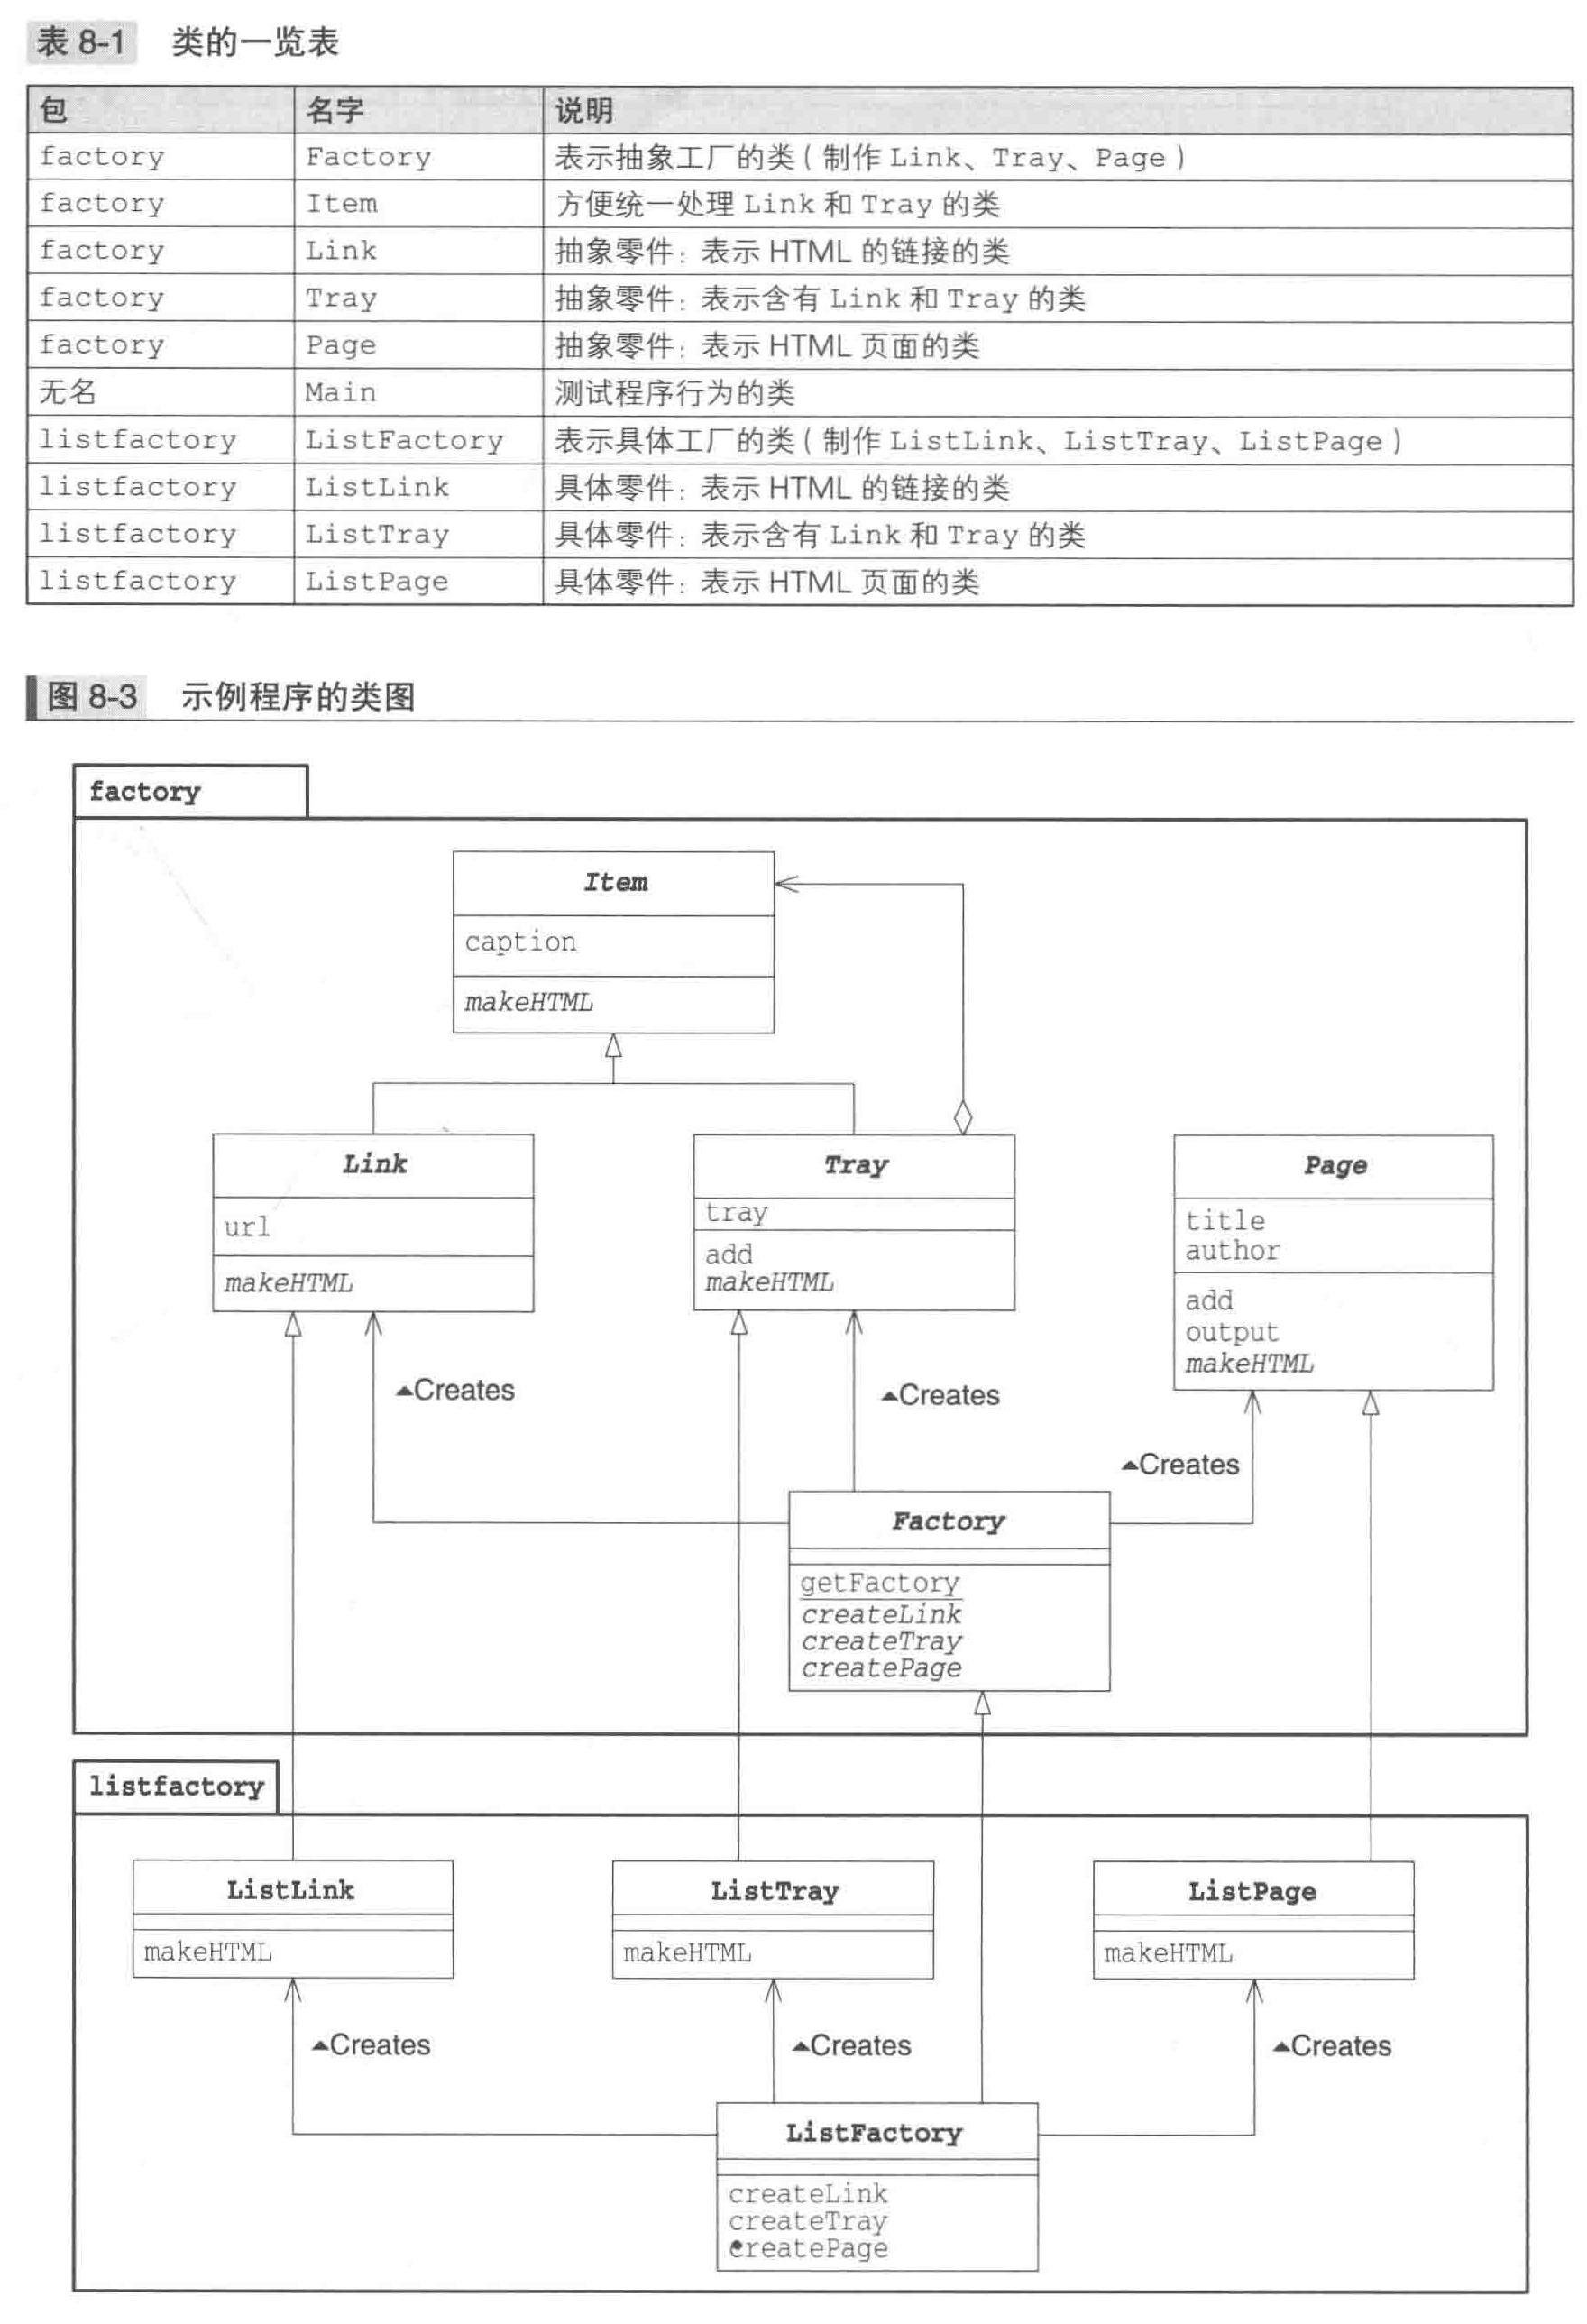
\includegraphics[width=\textwidth]{image/8-1}
\end{figure}
\subsection{factory}
\begin{lstlisting}
//代表项目,是 Link 和 Tray 的父类
public abstract class Item {
	//项目的标题
	protected String caption;
	public Item(String caption) {
		this.caption = caption;
	}
	public abstract String makeHtml();
}
\end{lstlisting}
\begin{lstlisting}
//表示 HYML 超链接的类
public abstract class Link extends Item {
	protected String url;
	public Link(String caption, String url) {
		super(caption);
		this.url = url;
	}
}
\end{lstlisting}
\begin{lstlisting}
//Tray 类表示一个含有多个 Link 类和 Tray 类的容器。
public abstract class Tray extends Item {
	protected List<Item> tray = new ArrayList<>();
	public Tray(String caption) {
		super(caption);
	}
	public void add(Item item) {
		tray.add(item);
	}
}
\end{lstlisting}
\begin{lstlisting}
//抽象地表示 HTML 页面的类,可以看作是零件组成的产品
public abstract class Page {
	protected String title;
	protected String author;
	protected List<Item> content = new ArrayList<>();
	public Page(String title, String author) {
		this.title = title;
		this.author = author;
	}
	public void add(Item item) {
		content.add(item);
	}
	public void output() {
		try {
			String fileNmae = title + ".html";
			Writer writer = new FileWriter(fileNmae);
			writer.write(this.makeHtml());
			writer.close();
			System.out.println(fileNmae + "编写完成");
		} catch (IOException e) {
			e.printStackTrace();
		}
	}
	public abstract String makeHtml();
}
\end{lstlisting}
\begin{lstlisting}
public abstract class Factory {
	public static Factory getFactory(String className) {
	Factory factory = null;
		try {
			factory = (Factory) Class.forName(className).newInstance();
		} catch (ClassNotFoundException e) {
			System.out.println("not found " + className + " class");
		} catch (Exception e) {
			e.printStackTrace();
		}
		return factory;
	}
	public abstract Link createLink(String caption, String url);
	public abstract Tray createTray(String caption);
	public abstract Page createPage(String title, String author);
}
\end{lstlisting}
\subsection{Main}
\begin{lstlisting}
public class Main {
	public static void main(String[] args) {
		Scanner scanner = new Scanner(System.in);
		String line = scanner.nextLine();
		Factory factory = Factory.getFactory(line);
		Link people = factory.createLink("人民日报", "http://www.people.com.cn");
		Link gmw = factory.createLink("光明日报", "http://www.gwm.cn/");
		Link us_yahoo = factory.createLink("Yahoo!", "http://www.yahoo.com/");
		Link jp_yahoo = factory.createLink("Yahoo! Japan", "http://www.yahoo.co.jp/");
		Link excite = factory.createLink("Excite", "http://www.excite.com/");
		Link google = factory.createLink("Google", "http://www.google.com/");
		
		Tray trayNews = factory.createTray("日报");
		trayNews.add(people);
		trayNews.add(gmw);
		
		Tray trayYahoo = factory.createTray("Yahoo!");
		trayYahoo.add(us_yahoo);
		trayYahoo.add(jp_yahoo);
		
		Tray traySearch = factory.createTray("搜索引擎");
		traySearch.add(trayYahoo);
		traySearch.add(excite);
		traySearch.add(google);
		
		Page page = factory.createPage("LinkPage", "杨文轩");
		page.add(trayNews);
		page.add(traySearch);
		page.output();
	}
}
\end{lstlisting}
\subsection{listfactory}
\begin{lstlisting}
public class ListLink extends Link {
	public ListLink(String caption, String url) {
		super(caption, url);
	}
	public String makeHtml() {
		return "    <li><a href=\"" + url + "\">" + caption + "</a><li>\n";
	}
}
\end{lstlisting}
\begin{lstlisting}
public class ListTray extends Tray {
	public ListTray(String caption) {
		super(caption);
	}
	public String makeHtml() {
		StringBuffer buffer = new StringBuffer();
		buffer.append("<li>\n");
		buffer.append(caption + "\n");
		buffer.append("<ul>\n");
		Iterator<Item> it = tray.iterator();
		while (it.hasNext()) {
			Item item = it.next();
			buffer.append(item.makeHtml());
		}
		buffer.append("</ul>\n");
		buffer.append("</li>\n");
		return buffer.toString();
	}
}
\end{lstlisting}
\begin{lstlisting}
public class ListPage extends Page {
	public ListPage(String title, String author) {
		super(title, author);
	}
	public String makeHtml() {
		StringBuffer buffer = new StringBuffer();
		buffer.append("<html><head><title>" + title + "</title></head>\n");
		buffer.append("<body>\n");
		buffer.append("<h1>" + title + "</h1>\n");
		buffer.append("<ul>\n");
		Iterator<Item> it = content.iterator();
		while (it.hasNext()) {
			Item item = it.next();
			buffer.append(item.makeHtml());
		}
		buffer.append("</ul>\n");
		buffer.append("<hr><address>" + author + "</address>");
		buffer.append("</body></html>\n");
		return buffer.toString();
	}
}
\end{lstlisting}
\begin{lstlisting}
public class ListFactory extends Factory {
	public Link createLink(String caption, String url) {
		return new ListLink(caption, url);
	}
	public Tray createTray(String caption) {
		return new ListTray(caption);
	}
	public Page createPage(String title, String author) {
		return new ListPage(title, author);
	}
}
\end{lstlisting}
\subsection{tablefactory}
\begin{lstlisting}
public class TableLink extends Link {
	public TableLink(String caption, String url) {
		super(caption, url);
	}
	public String makeHtml() {
		return "<td><a href=\"" + url + "\">" + caption + "</a></td>\n";
	}
}
\end{lstlisting}
\begin{lstlisting}
public class TableTray extends Tray {
	public TableTray(String caption) {
		super(caption);
	}
	public String makeHtml() {
		StringBuffer buffer = new StringBuffer();
		buffer.append("<td>");
		buffer.append("<table width=\"100%\" border=\"1\"><tr>");
		buffer.append("<td bgcolor=\"#cccccc\" align = \"center\" colspan=\"" + tray.size() + "\"><b>"
			+ caption + "</b></td>");
		buffer.append("</tr>\n");
		buffer.append("<tr>\n");
		Iterator<Item> it = tray.iterator();
		while (it.hasNext()) {
			Item item = it.next();
			buffer.append(item.makeHtml());
		}
		buffer.append("</tr></table>");
		buffer.append("</td>");
		return buffer.toString();
	}
}
\end{lstlisting}
\begin{lstlisting}
public class TablePage extends Page {
	public TablePage(String title, String author) {
		super(title, author);
	}
	public String makeHtml() {
		StringBuffer buffer = new StringBuffer();
		buffer.append("<html><head><title>" + title + "</title></head>\n");
		buffer.append("<body>\n");
		buffer.append("<h1>" + title + "</h1>\n");
		buffer.append("<table width=\"80%\" border =\"3\">\n");
		Iterator<Item> iterator = content.iterator();
		while (iterator.hasNext()) {
			Item item = iterator.next();
			buffer.append(item.makeHtml());
		}
		buffer.append("</table>\n");
		buffer.append("<hr><address>" + author + "</address>");
		buffer.append("</body></html>\n");
		return buffer.toString();
	}
}
\end{lstlisting}
\begin{lstlisting}
public class TableFactory extends Factory {
	public Link createLink(String caption, String url) {
		return new TableLink(caption, url);
	}
	public Tray createTray(String caption) {
		return new TableTray(caption);
	}
	public Page createPage(String title, String author) {
		return new TablePage(title, author);
	}
}
\end{lstlisting}
\section{扩展思路}
\begin{enumerate}
	\item 易于增加具体的工厂;
	\item 难以增加新的零件。
\end{enumerate}
\section{相关模式}

\begin{enumerate}
	\item Builder模式:抽象工厂模式通过调用抽象产品的接口(API)来组装抽象产品,生成具有复杂结构的实例;
	Builder是分阶段地制作复杂实例。
	\item Factory Method模式:抽象工厂中零件和产品的生成会使用工厂模式。
	\item Composite模式:有时抽象工厂会使用组合模式。
	\item Singleton模式:有时会用到单例模式。
\end{enumerate}
\section{生成实例的方法}
\subsection{new}
Something obj = new Something();
\subsection{clone}
复制新的实例。
\subsection{newInstance}
someobj.getClass().newInstance();